\usetikzlibrary{calc}
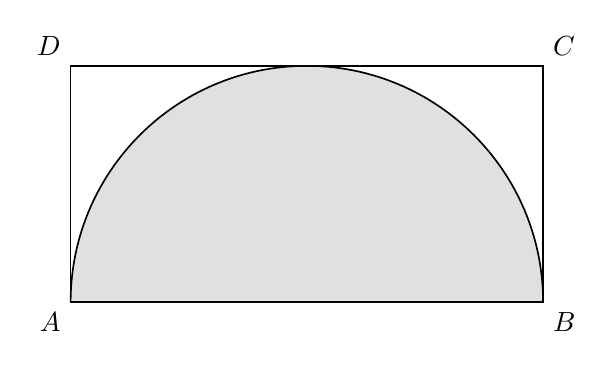
\begin{tikzpicture}[x=1cm,y=1cm,line width=.6pt,font=\normalsize]
\coordinate (A) at (0,0);
\coordinate (B) at (6,0);
\coordinate (C) at (6,3);
\coordinate (D) at (0,3);
\coordinate (O) at (3,0);
\fill[black!12] (A) arc[start angle=180,end angle=0,radius=3cm]--cycle;
\draw (A)--(B)--(C)--(D)--cycle;
\draw (A) arc[start angle=180,end angle=0,radius=3cm];
\node[below left] at (A) {$A$};
\node[below right] at (B) {$B$};
\node[above right] at (C) {$C$};
\node[above left] at (D) {$D$};
\end{tikzpicture}
